\chapter{Desenvolvimento}
	\chapterprecis{Este capítulo apresenta o desenvolvimento do sistema objetivo deste trabalho. São apresentadas as decisões de projeto, arquitetura e alguns trechos não triviais do códigos são explicados}
	
	\section{Decisões de Projeto}
		O estado atual do trocador de calor foi descrito na \autoref{sec:trocador}. O intuito deste projeto é implementar um sistema de monitoramento e controle remoto sem que haja alteração da infraestrutura já instalada. Em resumo, o objetivo é incluir algum dispositivo que necessite apenas se comunicar com o Arduino para executar suas tarefas.
		
		Para este projeto, é possível utilizar tanto uma arquitetura SCADA tradicional, quanto tecnologias embarcadas como placas de prototipagem. Foi definido utilizar a segunda opção, devido a fatores econômicos e também pela portabilidade concedida ao sistema. A arquitetura foi inspirada em grande parte no sistema BrewPi, descrito na \autoref{sec:exemplos}. O Raspberry Pi 3 foi escolhido por possuir comunicação Wifi integrada à placa, e possuir uma documentação mais extensa que outras placas similares no mercado como o BeagleBone Black\footnote{\url{https://beagleboard.org/black}} e a recente e também poderosa placa DragonBoard 410c\footnote{\url{https://developer.qualcomm.com/hardware/dragonboard-410c}}. Dessa forma, a visão geral do sistema proposto é exibida na \autoref{fig:arq_proposta}.
		
		\begin{figure}[!htb]	
			%\centering
			\captionsetup{justification=centering}
			\begin{center}
				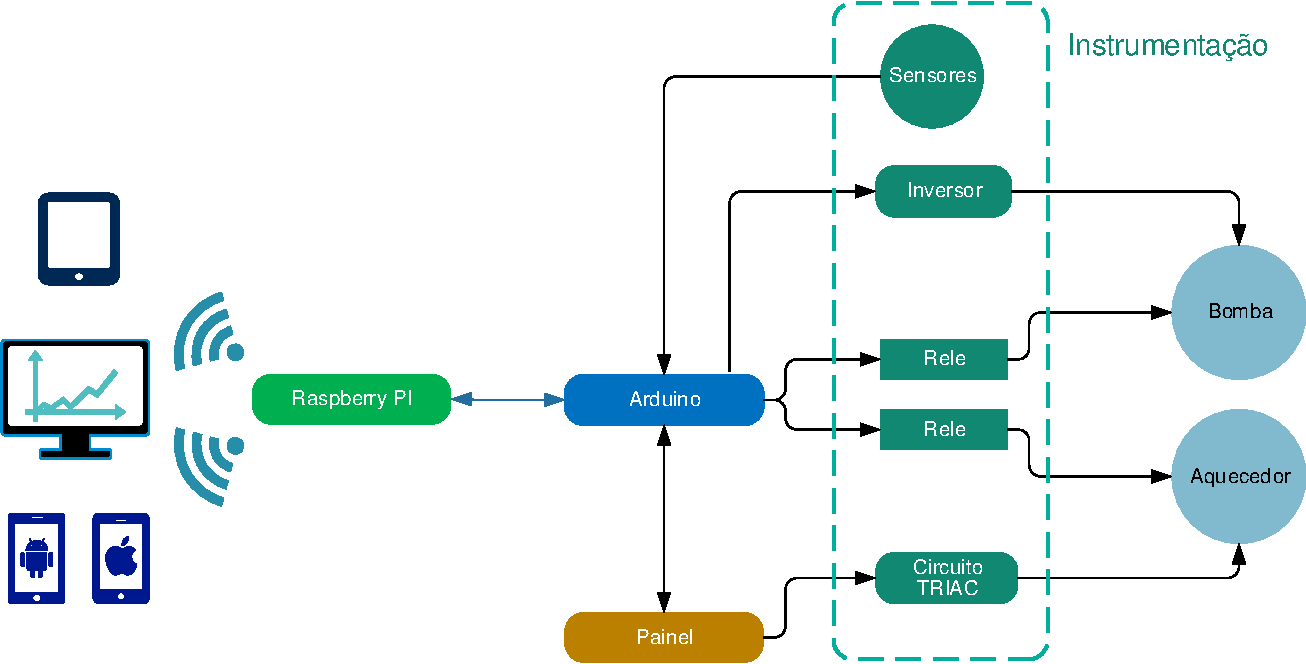
\includegraphics[width=14cm]{arq_proposta}  %pode alterar o tamanho
				\caption[Nova Arquitetura Proposta para o Sistema]{\label{fig:arq_proposta} Nova Arquitetura Proposta para o Sistema }
			\end{center}	
		\end{figure}
	
	\section{Requisitos Funcionais do Sistema}
		Uma vez definido o hardware a ser utilizado, deve-se levantar os requisitos funcionais do sistema, ou seja o que o sistema deve fazer e como deve reagir em determinadas situações. Basicamente, os requisitos funcionais são as características de operação do sistema de monitoramento a ser desenvolvido. Os requisitos estão resumidos na \autoref{tbl:requisitos}.
			
		\begin{table}[!htb]
			\centering
			\caption{Requisitos Funcionais do Sistema}
			\label{tbl:requisitos}
			\def\arraystretch{1.3}
			\begin{tabular}{c p{11cm}}
				\hline
				\multicolumn{1}{c}{\textbf{Índice Requisito}} & \multicolumn{1}{c}{\textbf{Descrição Requisito}} \\ \hline 
				1 & Exibir a informação atual das variáveis de processo (vazões e temperaturas) \\ %\hline
				2 & Exibir o estado da bomba e do aquecedor (Ligado ou Desligado) \\ %\hline  
				3 & Exibir o valor da rotação atual da bomba \\ %\hline
				4 & Em modo remoto, deve permitir que o operador acione a bomba e o aquecedor \\ %\hline
				5 & Em modo remoto, deve permitir que o operador altere a velocidade da bomba \\ %\hline
				6 & Permitir a visualização dos dados analógicos em gráficos \\ %\hline
				7 & Impedir a atuação do operador quando o Arduino estiver em modo local ou de emergência \\ %\hline
				8 & Armazenar os dados do sistema em banco de dados \\ %\hline
				9 & Permitir que o usuário habilite ou desabilite o armazenamento de dados das variáveis \\ %\hline
				10 & Permitir que o usuário colete as informações contidas no banco em um arquivo no formato csv \\ %\hline
				11 & Permitir que o usuário apague as informações contidas no banco de dados \\ \hline
			\end{tabular}
		\end{table}
		
		\subsection{Descrição Funcional}
			\label{sec:desc_funcional}
			Para atender aos requisitos citados acima, optou-se por modularizar as funcionalidades do sistema. Dessa forma, foram definidos 3 componentes. O termo componente deve ser entendido como um programa. Os componentes foram projetados de forma que cada um funcione de forma mais independente possível. Assim, o impacto no sistema caso haja alguma alteração de componente, em termos de reengenharia, é minimizado.
			
			A relação entre os componentes é exibida na  \autoref{fig:arq_componentes}. Foram definidos 3 componentes: o programa que é executado no Arduino; o Gateway e o WebServer, que são programas executados no Raspberry. Optou-se por criar dois componentes no Raspberry PI, de forma que as funcionalidades do sistema fossem corretamente agrupadas. As atribuições de cada programa estão resumidas na \autoref{tbl:atribuições}.
			
			\begin{figure}[!htb]	
				%\centering
				\captionsetup{justification=centering}
				\begin{center}
					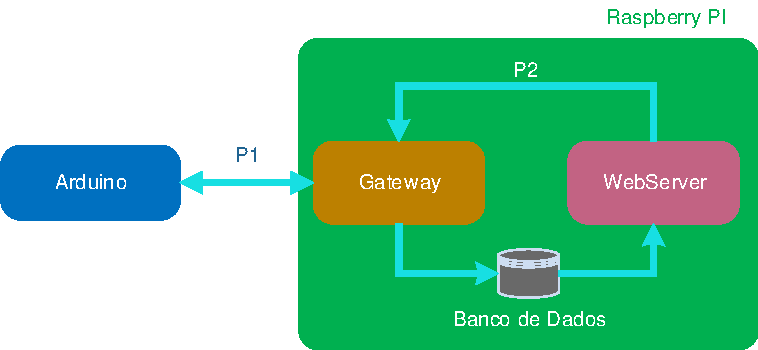
\includegraphics[scale=0.7]{arq_componentes}  %pode alterar o tamanho
					\caption[Arquitetura Detalhada]{\label{fig:arq_componentes} Arquitetura Detalhada }
				\end{center}		
			\end{figure}
			
			\begin{table}[!htb]
				\centering
				\captionsetup{justification=centering}
				\caption[Atribuições de cada Componente]{Atribuições de cada Componente}
				\label{tbl:atribuições}
				\def\arraystretch{1.3}
				\begin{tabular}{m{2cm}| p{12cm}}
					\hline
					& \multicolumn{1}{c}{\textbf{Atribuições}} \\ \hline
					
					\multirow{4}{*}{Arduino} 
					& 1 - Interface com sensores e Atudadores \\
					& 2 - Interface com Painel \\
					& 3 - Enviar estado do sistema quando solicitado pelo Gateway\\
					& 4 - Interpretar comandos enviados pelo Gateway \\ \hline
					
					\multirow{3}{*}{Gateway} & 5 - Solicitar de forma cíclica o estado das variáveis \\
					& 6 - Armazenar os dados recebidos em um banco de dados \\
					& 7 - Receber comandos vêm do WebServer (comandos dos usuários) e repassar ao Arduino \\ \hline
					
					\multirow{2}{*}{WebServer} & 8 - Ler dados do banco e apresentar ao usuário \\
					& 9 - Receber comandos do usuário e repassar ao Gateway \\
					
					\hline
				\end{tabular}
			\end{table}
		
			É importante observar que o Gateway apenas cuida da transferência de informações entre WebServer e Gateway. O programa contém duas threads: uma para realizar a solicitação cíclica de dados ao Arduino e armazená-los no banco de dados; e a outra para aguardar o envio de comandos vindos do WebServer e repassar ao Arduino.  A comunicação entre Gateway e Arduino é realizada através do protocolo I2C, e a comunicação entre Gateway e WebServer é feita através de sockets TCP/IP.
			
			O sistema foi projetado de forma que a substituição de um componente não influencie os demais, contudo alterações nos protocolos influenciaria o código dos componentes envolvidos. Portanto os protocolos devem ser mantidos.
			 
	\section{Implementação}
		Essa seção consiste em detalhar o funcionamento dos componentes e a comunicação entre eles. Alguns trechos de códigos, considerados não triviais são explicados.
		
		\subsection{Arduino}
			\label{Arduino}
			O código fonte completo está disponibilizado no Github\footnote{\url{https://www.oficinadanet.com.br/post/14791-o-que-github}}, no link \url{https://github.com/felipefonsecabh/ArduinoCode/blob/ArduinoNoNavigation/ArduinoCode.ino}
			
			Foi feita uma análise do programa atual que o Arduino executa. O programa é extenso (contém 1482 linhas), sendo que cerca de 90\% do código é dedicado a cuidar do sistema de navegação do display LCD através dos botões existentes no painel.  A implementação de um sistema de monitoramento elimina a necessidade dessa estrutura de navegação, de modo que o painel passe a ter apenas funcionalidades diretas de acionamento, e o display exiba apenas informações básicas. Portanto, a melhor opção foi reformular o código do Arduino e aproveitar apenas as funções que fazem a leitura dos sensores e convertem os valores para unidade de engenharia. Essas funções se fazem necessária, pois não é escopo do projeto recalibrar sensores e/ou alterar a instrumentação já existente.
				
			A estrutura do código, que está exibida na \autoref{fig:fluxo_arduino}, foi montada de forma a permitir rápida adaptação do mesmo para diferentes protocolos de comunicação, e está de acordo com as atribuições mencionadas na \autoref{tbl:atribuições}. As trocas de mensagens com o Gateway são feitas por interrupção, ou seja, estão fora da função \textit{loop} do Arduino. 
				
			O programa foi intensamente modularizado. Todos os estados e funcionalidades foram encapsuladas em funções. Esse tipo de prática acelera a interpretação do código. Outro benefício é a possibilidade de expansão de funcionalidades, como por exemplo a implementação de malhas de controle no código. 
				
			No diagrama é utilizado o termo ``estado do sistema'', que deve ser interpretado como o conjunto de variáveis necessários para descrever o sistema. Essas variáveis são: as 4 temperaturas; 2 vazões; estado de acionamento de bomba e aquecedor (Ligado ou Desligado); velocidade da bomba; modo de operação (Local ou Remoto) e se o botão de emergência está acionado ou não.
			
			\begin{figure}[!htb]	
					%\centering
					\captionsetup{justification=centering}
					\begin{center}
						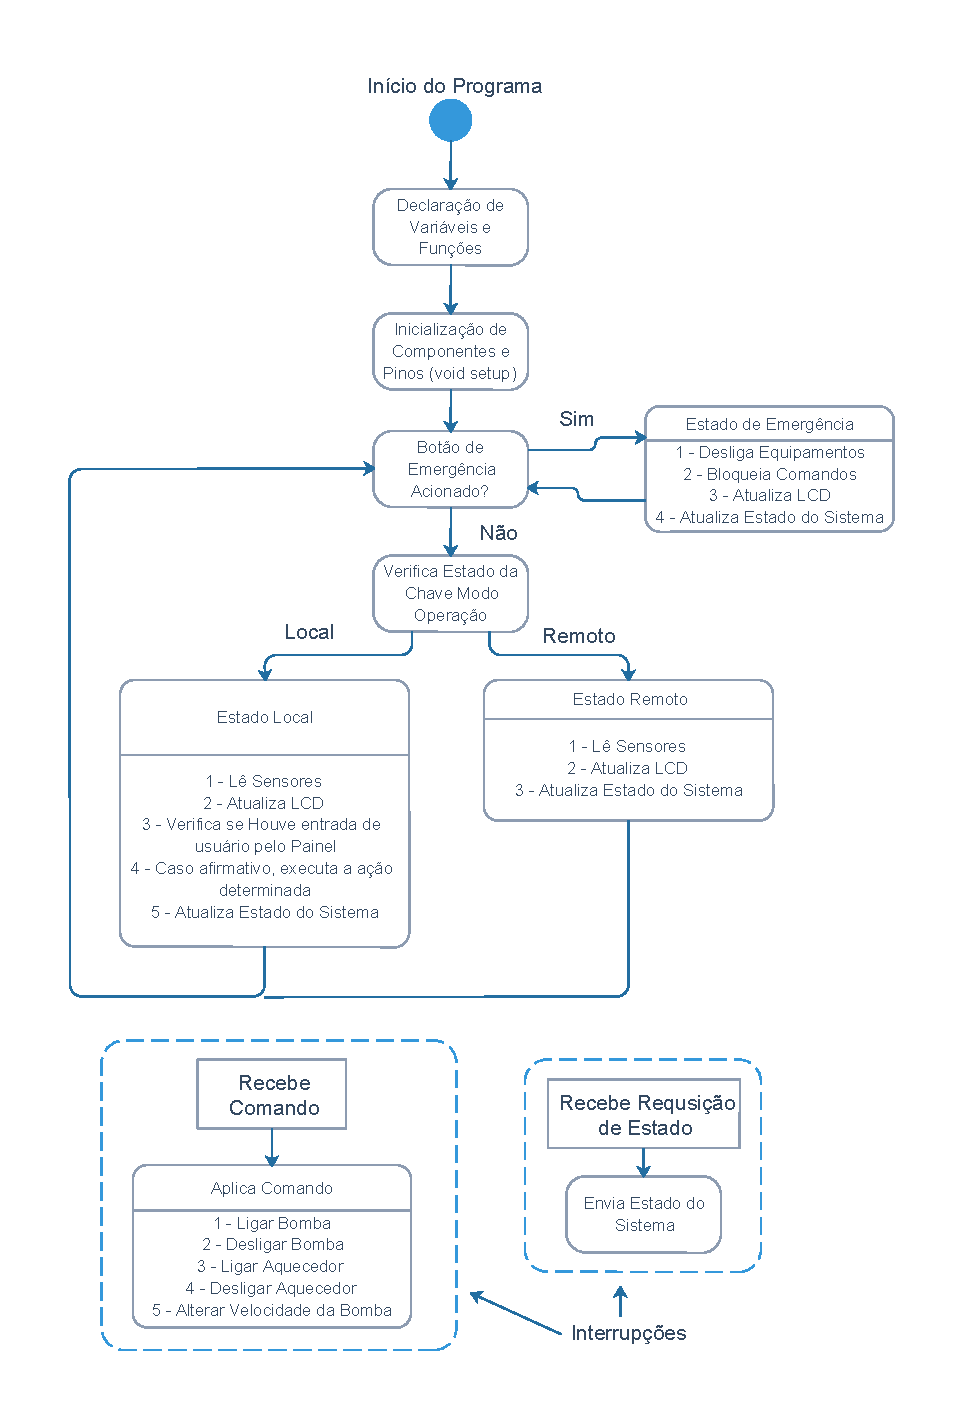
\includegraphics[width=12cm]{fluxo_arduino}  %pode alterar o tamanho
						\caption[Estrutura do Código do Arduino]{\label{fig:fluxo_arduino} Estrutura do Código do Arduino }
					\end{center}		
			\end{figure}
			
			Para a leitura dos sensores foram utilizadas bibliotecas desenvolvidas e mantidas por terceiros. A \autoref{tbl:libs} mostra a relação entre tabelas, desenvolvedores e versões. Não foi necessária nenhuma biblioteca para a leitura da vazão de água fria. O sensor de vazão consiste em um dispositivo que envia pulsos ao Arduino. Quanto mais pulsos enviados, maior é a vazão. Portanto, é feita uma contagem de pulsos em um intervalo de tempo fixo, e posteriormente esse número é inserido em uma fórmula que retorna o valor da vazão. A contagem de pulsos é feita por interrupção.
			
			O código correspondente a leitura dos valores analógicos é mostrado no \autoref{cod:read_arduino}.
			
			\begin{table}[!htb]
				\centering
				\captionsetup{justification=centering}
				\caption[Bibliotecas utilizadas no programa do Arduino]{Bibliotecas utilizadas no programa do Arduino}
				\label{tbl:libs}
				\def\arraystretch{1.3}
				\begin{tabular}{l c l l}
					\hline
					\textbf{Biblioteca} & \textbf{Versão}& \textbf{Mantida por} & \textbf{Função} \\ \hline
					Dallas Temperature & v3.7.6 & \textcite{miles2016} & Temperatura \\
					OneWire & v2.3.3 & \textcite{paul2017} & Temperatura \\
					Ultrasonic & - & \textcite{filipeflop2011} & Vazão Quente \\					
					\hline
				\end{tabular}
			\end{table}
		
			\begin{listing}[!htb]
				\begin{minted}[bgcolor=bg,breaklines=true,tabsize=2, baselinestretch=1,fontsize=\footnotesize]{cpp}
				void Temperaturas() {
					// call sensors.requestTemperatures() to issue a global temperature 
					// request to all devices on the bus
					sensors.requestTemperatures();
				
					// print the device information
					for (byte i = 0; i <= 4; i++){
						temp[i] = sensors.getTempC(deviceID[i]);
					}
				}
				
				void VazaoAguaFria(){
					currentTime = millis();
					// Every second, calculate litres/hour
					if (currentTime >= (cloopTime + 1000)){
						cloopTime = currentTime; // Updates cloopTime
						// Pulse frequency (Hz) = 7.5Q, Q is flow rate in L/min.
						vazao_fria = (flow_frequency / 7.5); // (Pulse frequency) / 7.5Q = flowrate in L/min
						flow_frequency = 0; // Reset Counter
					}
				}
				
				void VazaoAguaQuente(){
					float vazao1_sf; //descobrir o porque do nome da variavel
					microsec = ultrasonic.timing();
					cmMsec = ultrasonic.convert(microsec, Ultrasonic::CM);
					nivel = 11.46 - cmMsec;
					vazao1_sf = (0.0537)* pow((nivel * 10), 1.4727);
					if (vazao1_sf > 1){
						vazao_quente = 0.75*vazao_quente + 0.25*vazao1_sf;
					}
				}	
				\end{minted}
				\caption{Funções de Leitura dos sensores}
				\label{cod:arduino}
			\end{listing}
			
			A troca de dados entre Arduino e Gateway é feita pelo protocolo I2C. Este protocolo é implementado no Arduino através da biblioteca Wire. Neste projeto o Arduino atua como slave da comunicação, ou seja, não inicia a comunicação. Responde a algum dispositivo mestre apenas quando solicitado.
			 
			Quando o mestre envia um comando de escrita, atua-se uma interrupção, que executa a função onReceive. Quando o mestre envia uma solicitação de dados, atua-se uma outra interrupção, que executa a função onReceive e posteriormente executa a função onRequest. Em suma, a função onReceive é utilizada para interpretar comandos, como por exemplo ligar ou desligar bomba e aquecedor, e a função onRequest é utilizada para enviar para o mestre dados sobre o processo como por exemplo valores de temperaturas e vazões.
			
			As informações no protocolo I2C trafegam sob a forma de um array de bytes. Portanto, as informações referentes ao sistema, que são booleanas e reais, devem ser convertidas em um array de bytes para serem transmitidas.  É possível realizar essa conversão utilizando a declaração union. Essa técnica permite que variáveis de diferentes tipos ocupem uma mesma região de memória. Assim, foi criada uma estrutura de dados para representar o estado do sistema, que compartilha essa região de memória com um array de bytes. O \autoref{cod:dadosi2c} corresponde a essa implementação feita.
			
			\begin{listing}[!htb]
				\begin{minted}[bgcolor=bg,breaklines=true,tabsize=2, baselinestretch=1,fontsize=\footnotesize]{cpp}
				//estrutura de dados para envio i2c
				typedef struct processData{
					float temp1;
					float temp2;
					float temp3;
					float temp4;
					float hotflow;
					float coldflow;
					float pump_speed;
					byte bstatus;
					byte chksum;
				};
				
				typedef union I2C_Send{ //compartilha a mesma área de memória
					processData data;
					byte I2C_packet[sizeof(processData)];
				};				
				\end{minted}
				\caption{Estrutura de dados do sistema}
				\label{cod:dadosi2c}
			\end{listing}
			
			Em relação ao recebimento de comandos pelo Gateway, primeiramente é necessário entender como é a estrutura de um frame enviado pelo mestre. A estrutura do frame está descrita na \autoref{fig:i2c_packet}.
			
			\begin{figure}[!htb]	
				%\centering
				\captionsetup{justification=centering}
				\begin{center}
					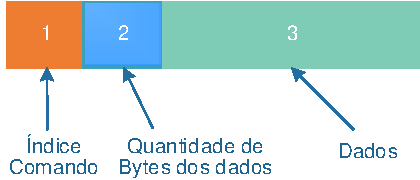
\includegraphics[scale=0.9]{i2c_packet}  %pode alterar o tamanho
					\caption[Estrutura de um pacote I2C]{\label{fig:i2c_packet}Estrutura de um pacote I2C}
				\end{center}		
			\end{figure}
		
			O índice de comando arbitrário e é definido pelo desenvolvedor. Portanto, para interpretar corretamente os comandos pelo mestre, foi necessário mapear ações de acordo com o índice de comando criado, ou seja, definir um protocolo básico de comunicação. A relação entre o índice de comando e a ação correspondente é mostrada na \autoref{tbl:comandos}. A interpretação e execução dos comandos é feita na função onReceive. Se o comando é uma solicitação de dados, o envio é realizado na função onRequest.
			
			\begin{table}[!htb]
				\centering
				\caption{Definição das interpretações de comando}
				\label{tbl:comandos}
				\def\arraystretch{1.3}
				\begin{tabular}{c c l}
					\hline
					\textbf{Comando (Char)} & \textbf{Comando (Decimal)} & \textbf{Ação}  \\ \hline
					
					`1' & 49 & Ligar a bomba \\ %\hline
					`2' & 50 & Desligar a bomba \\ %\hline  
					`3' & 51 & Ligar aquecedor \\ %\hline
					`4' & 52 & Desligar o aquecedor \\ %\hline
					`5' & 53 & Alterar velocidade da bomba \\
					`6' & 54 & Enviar dados do sistema para o mestre \\ %\hline
					\hline
				\end{tabular}
			\end{table}
		
		Foi colocada a representação decimal e em char dos comandos, porque no Arduíno o comando é interpretado na forma decimal, enquanto no Gateway os comandos são interpretados como char. A relação entre o valor em char e decimal é dada pela tabela ASCII\footnote{\url{https://en.wikipedia.org/wiki/ASCII}}.
		
	\subsection{Preparação do Raspberry}
		\subsubsection{Instalação do sistema operacional}
		O Raspberry não possui memória de armazenamento interna. Portanto, é necessário instalar o sistema operacional (SO) em um microUSB, que faz o papel de HD. Foi utilizada o SO ``Raspian Stretch With Desktop'', disponível no link \url{https://www.raspberrypi.org/downloads/raspbian/}. Basicamente, deve-se extrair a imagem baixada para o microUSB. Após esse procedimento o Raspberry Pi já pode ser inicializado.
		
		\subsubsection{Ativação do protocolo I2C e Conexão com Arduíno}
		O I2C não vem habilitado por padrão no sistema operacional. É necessário entrar nas configurações do Rpi e habilitá-lo. Os passos para realizar esse procedimento estão descritos por \textcite{matt2014}. 
		
		Após ativar o protocolo, é necessário conectar o Raspberry com o Arduíno. A ligação é feita através de dois fios, e ainda o fio para interligar o terra. A \autoref{tbl:conn_rpi_arduino} mostra com os pinos devem ser interligados.
		
		\begin{table}[!htb]
			\centering
			\caption{Ligação I2C entre Raspberry e Arduíno}
			\label{tbl:conn_rpi_arduino}
			\def\arraystretch{1.3}
			\begin{tabular}{c c}
				\hline
				\multicolumn{1}{c}{\textbf{Raspberry}} & \multicolumn{1}{c}{\textbf{Arduino}} \\ \hline
				
				Pino 3 & Pino 20 \\
				Pino 5 & Pino 21 \\ %\hline
				Pino 9 & Gnd \\ %\hline  
				\hline
			\end{tabular}
		\end{table}
		
		\subsubsection{Instalação de Pacotes - Python}
		O sistema operacional Raspian já possui duas versões instaladas de Python: 2.7 e 3.4. A primeira, mesmo sendo mais antiga ainda é muito utilizada pela comunidade devido à grande quantidade de pacotes desenvolvidos para essa versão; a segunda, é uma das versões mais novas disponíveis para Python.
		
		Os códigos do Gateway e do WebServer foram desenvolvidos com a versão 3.4. Antes do começo do desenvolvimento é necessário instalar os pacotes necessários para executar o projeto. Os pacotes a serem instalados dependem do propósito e característica do sistema a ser desenvolvido. É muito comum desenvolvedores trabalharem em diferentes projetos, portanto a tarefa de gerenciar os pacotes para cada projeto torna-se trabalhosa. Para isso, o Python disponibiliza a instalação de ambientes virtuais na máquina. Ambientes virtuais são diretórios para armazenar os pacotes necessários para determinados projetos. Assim, é possível isolar os arquivos de cada desenvolvimento, facilitando a mudança de um projeto para o outro \cite{kyle2017}. A utilização de ambientes virutais em Python é uma boa prática de programação e foi utilizada.
		
		Para instalar um ambiente virtual na versão python 3, é necessário utilizar os comandos descritos no \autoref{cod:venv}. Uma vez instalado, é necessário ativar o ambiente virtual, cujo comando é exibido no \autoref{cod:activate_venv}. Após ativado, devem-se instalar os pacotes necessários para o projeto. Os pacotes e as versões instaladas estão listados na \autoref{tbl6}. Todos os pacotes, com exceção do Smbus, podem ser instalados através do comando exibido no \autoref{cod:install}. É necessário ativar o ambiente virtual antes de efetuar os comandos. Para a instalação do Smbus, é necessário seguir os passos descritos por \textcite{dipto2015}.
		
		\begin{listing}[!htb]
			\begin{minted}[bgcolor=bg,breaklines=true,tabsize=2, baselinestretch=1,fontsize=\footnotesize]{bash}
			#navegar até a pasta onde se deseja instalar o ambiente virtual
			pi@raspberry $ cd pfc_env
			
			#instalar pacote virtual env
			pi@raspberry $ pip install virtualenv
			
			#criar um ambiente virtual chamado env
			pi@raspberry $ virtual env			
			\end{minted}
			\caption{Comandos para criação de um ambiente virtual}
			\label{cod:venv}
		\end{listing}
		
		\begin{listing}[!htb]
			\begin{minted}[bgcolor=bg,breaklines=true,tabsize=2, baselinestretch=1,fontsize=\footnotesize]{bash}
			#ativar o diretório virtual
			pi@raspberry $ source pfc_env/bin/activate
			
			#caso o nome do diretório apareça entre parenteses como abaixo, o diretório foi ativado com sucesso
			(env) pi@raspberry $ 		
			\end{minted}
			\caption{Comandos para criação de um ambiente virtual}
			\label{cod:activate_venv}
		\end{listing}
		
		
		\begin{table}[!htb]
			\centering
			\caption{Pacotes necessários para o projeto}
			\label{tbl6}
			\def\arraystretch{1.3}
			\begin{tabular}{c c}
				\hline
				\multicolumn{1}{c}{\textbf{Pacote}} & \multicolumn{1}{c}{\textbf{Versão}} \\ \hline
				
				Smbus & v1.9.2 \\
				Django & v1.9.2 \\ %\hline
				Pillow & v1.9.2 \\ %\hline  
				\hline
			\end{tabular}
		\end{table}
		
		\begin{listing}[!htb]
			\begin{minted}[bgcolor=bg,breaklines=true,tabsize=2, baselinestretch=1,fontsize=\footnotesize]{bash}
			#ativar o diretório virtual
			#o comando é pip install NomePacote== Versão. Exemplo:
			(env) pi@raspberry $ pip install Django==1.9.6					
			\end{minted}
			\caption{Comando para a instalação de pacotes Python}
			\label{cod:install}
		\end{listing}
		
	\subsection{Gateway}
		O código fonte completo do gateway está disponibilizado no Github, no link: \url{https://github.com/felipefonsecabh/PFC/blob/PyServeri2c/arduinoserver.py}. Conforme mencionado na \autoref{sec:desc_funcional}, o programa consiste em 2 threads que são executadas continuamente, ou seja em loop infinito.
		
		\subsubsection{Thread 1: Leitura de Dados do Arduino e Escrita no Banco}
		Para implementar a comunicação I2C no Gateway, utiliza-se a biblioteca Smbus. Primeiramente é necessário inicializar a conexão com o Arduino, referenciando o endereço do mesmo. Esse endereço é arbitrário, e deve possuir o mesmo valor no código do Arduino e no Gateway. Foi escolhido o identificador 12 para o endereço do Arduino.
		
		\begin{listing}[!htb]
			\begin{minted}[bgcolor=bg,breaklines=true,tabsize=2, baselinestretch=1,fontsize=\footnotesize]{python}
			#inicialização do i2c
			bus = SMBus(1)
			arduinoAddress = 12				
			\end{minted}
			\caption{Inicialização da comunicação I2C}
			\label{cod:starti2c}
		\end{listing}
		
		A solicitação de dados para o Arduino foi feita através da utilização da função read\_i2c\_block\_data. É necessário passar como parâmetro o endereço do Arduino, o ínidice do comando (foi definido na \autoref{tbl:comandos} que o índice do comando da solicitação de dados era 54), e o número de bytes esperados na resposta. O resultado retorna um array de bytes que deve ser convertido nas variáveis reais de processo. Para realizar essa conversão foi utilizada a função unpack do pacote struct\footnote{\url{https://docs.python.org/2/library/struct.html}}. Um exemplo de pacote recebido do Arduino é mostrada na \duvida{figuraX}.
		
		Portanto, é necessário separar o array de bytes em 7 variáveis float e 2 variáveis do tipo byte. O primeiro byte contém as informações de status digitais, e o segundo byte é apenas um valor para verificação da integridade do pacote. Após a separação em variáveis, os dados foram organizados em um dicionário\footnote{Como funciona um dicionário: \cite{mark2013}} para facilitar o envio para o banco.
		
		\begin{listing}[!htb]
			\begin{minted}[bgcolor=bg,breaklines=true,tabsize=2, baselinestretch=1,fontsize=\footnotesize]{python}
			#faz requisicao pelos dados
			block = bus.read_i2c_block_data(arduinoAddress,54,30)
			#conversao do array de bytes em variaveis
			data = unpack('7f2b',bytes(block))
			#inserção dos dados em um dicionário
			bstatus, lastdata, lasttrenddata = parseData(data)			
			\end{minted}
			\caption{Leitura dos dados do Arduino}
			\label{cod:read_arduino}
		\end{listing}
		
		O banco de dados possui 3 tabelas: uma tabela para armazenar o estado mais recente do sistema chamada Registers, outra tabela para armazenar o histórico das variáveis chamada TrendRegisters, e uma tabela para armazenar variáveis de controle (como o modo de operação do sistema por exemplo, e se o armazenamento histórico deve estar habilitado ou não) chamada OperationMode. Para armazenar dados no banco, primeiramente é necessário estabelecer uma conexão com o banco (ver \autoref{cod:connect_bd}). A inserção do dado no banco consiste em acessar a tabela passando como parâmetro o dicionário criado anteriormente; por fim, deve-se executar o método save para concluir a operação (ver \autoref{cod:insert_data}).
		
		\begin{listing}[!htb]
			\begin{minted}[bgcolor=bg,breaklines=true,tabsize=2, baselinestretch=1,fontsize=\footnotesize]{python}
			#estabelece conexão com o banco de dados
			if os.environ.setdefault('DJANGO_SETTINGS_MODULE', 'WebSite.settings'):
				import django
				django.setup()
				from WebSite.operation.models import Registers, OperationMode
				from WebSite.trend.models import TrendRegister
				from django.utils import timezone
			else:
				raise
				sys.exit(1)
			\end{minted}
			\caption{Conexão com o banco de dados}
			\label{cod:connect_bd}
		\end{listing}
		
		\begin{listing}[!htb]
			\begin{minted}[bgcolor=bg,breaklines=true,tabsize=2, baselinestretch=1,fontsize=\footnotesize]{python}
			#envia dado para o banco de dados (lastdata contém últimos dados válidos)
			reg = Registers(**lastdata)
			reg.save()
			
			#envia dado para o banco de dados
			treg = TrendRegister(**lasttrenddata)
			treg.save()
			\end{minted}
			\caption{Código necessário para inserção de dados no banco}
			\label{cod:insert_data}
		\end{listing}
		
		As operações de leitura de banco de dados e escrita no banco são cíclicas, ou seja, executam a cada intervalo de tempo. O intervalo das operações é definido no início do código fonte. O tempo é determinado em milissegundos.
		
		\begin{listing}[!htb]
			\begin{minted}[bgcolor=bg,breaklines=true,tabsize=2, baselinestretch=1,fontsize=\footnotesize]{python}
			#intervalo de execução das operações
			start_time = datetime.now()
			readinterval = 100        #intervalo de leitura do arduino
			sendDBinterval = 600      #intervalo de gravação na tabela Registers
			sendTrendDBinterval = 300 #intervalo de gravação na tabela TrendRegisters
			\end{minted}
			\caption{Intervalo de execução das operações}
			\label{cod:set_interval}
		\end{listing}
		
		\subsubsection{Thread 2: Recebimento de Comandos do WebServer}
		A segunda thread implementa um servidor TCP que fica escutando na porta 8080. O servidor TCP implementado é assincrono, ou seja, não bloqueiam o processo em que estão sendo executados enquanto aguardam dados de algum cliente. Quando algum dado chega, é chamada uma função callback para processá-lo \cite{pythondoc}. Foi utilizado o pacote asyncore, que é disponibilizado na instalação padrão do Python para implementar o servidor assíncrono. A função callback chamada para interpretar os pacotes é a handle\_read, mostrada no \autoref{cod:handle_read}
		
		O WebServer envia comandos de duas formas. A primeira, envia apenas um byte, que é o código de comando a ser executado (ligar bomba, apagar histórico, entre outros); a função process\_commands executa as ações necessárias de acordo com o comando recebido. A segunda forma, envia um pacote JSON\footnote{O que é JSON: \url{http://json.org/}}, que contém o valor da velocidade da bomba a ser setada. O pacote JSON é processado, e o valor da velocidade é enviado para o Arduino na forma de um array de bytes.
		
		\begin{listing}[!htb]
			\begin{minted}[bgcolor=bg,breaklines=true,tabsize=2, baselinestretch=1,fontsize=\footnotesize]{python}
			def handle_read(self):
				#recebe dado do cliente
				data = self.recv(50)
				if len(data) < 2:  #comandos digitais
					process_commands(data)
				else: #comando analogico
					try:
						#Exemplo de pacote JSON
						'{"pump_speed": 85.4}'
			
						ld = json.loads(data.decode('utf-8'))
						bytescommand = pack('f',ld['pump_speed'])
						bus.write_block_data(arduinoAddress,53,list(bytescommand))
					except Exception as err:
						print(str(err))
					finally:
						pass
			\end{minted}
			\caption{Função que interpreta comandos vindos do WebServer}
			\label{cod:handle_read}
		\end{listing}
	
	\subsection{WebServer}
	O código fonte completo do WebServer está disponibilizado no Github, no link: \url{https://github.com/felipefonsecabh/PFC}. Ao contrário dos códigos anteriores, o projeto do WebServer é composto de múltiplos arquivos.
	
	A estrutura de um projeto django segue a estrutura mostrada na \autoref{fig:django_project}. Um projeto é composto de várias aplicações (apps). Uma aplicação pode ser entendida como um módulo do programa, ou seja, um trecho que possui um conjunto de funcionalidades específicas e funciona de forma independente. A utilização de múltiplas apps no projeto é incentivada, pois permite o desenvolvimento de um sistema pouco acoplado.
	
	A \autoref{fig:django_project} também mostra os arquivos que compõem uma aplicação. Destacam-se os aqueles que implementam o modelo MVC. Os arquivos de modelo implementam as estruturas de dados a serem utilizadas na aplicação. Cada estrutura de dados (classe) é mapeada na forma de uma tabela no banco de dados, e cada instância dessa estrutura na aplicação é uma linha na tabela criada, implementando assim o ORM, como mencionado na \autoref{sec:django}.
	
	Os arquivos urls e views implementam a parte do processamento de requisições do usuário e processo de apresentação de conteúdo. O arquivo url contém o mapeamento entre os recursos e as funções que devem ser executadas. Quando uma url é chamada, esse mapeamento é consultado e assim é chamada a função especificada.
	
	As funções estão no arquivo views, que fazem o processamento propriamente dito. Basicamente, quando uma view é chamada, ela efetua operações com os modelos de dados quando necessário e retorna para o usuário algum arquivo de template.
	
	Os templates são basicamente arquivos html que aceitam comandos disponibilizados pelo Framework para que se possa adicionar conteúdo dinâmico ao arquivo, antes de enviá-lo para o usuário. Alguns dos comandos mais utilizados são: exibir variáveis, cujos valores são preenchidos pelas views, ``inserir templates dentro de outros'', o que possibilita reaproveitamento de código, comandos de decisão (if, else), de fluxo (for) entre outros. Os comandos possuem a sintaxe  \{\% comando \%\}, exceto as variáveis, que são definidas por \{\{ variável \}\}. O fluxo de informações entre o usuário e uma aplicação django é exibido na \autoref{fig:fluxo_django}
	
	\begin{figure}[!htb]	
		%\centering
		\captionsetup{justification=centering}
		\begin{center}
			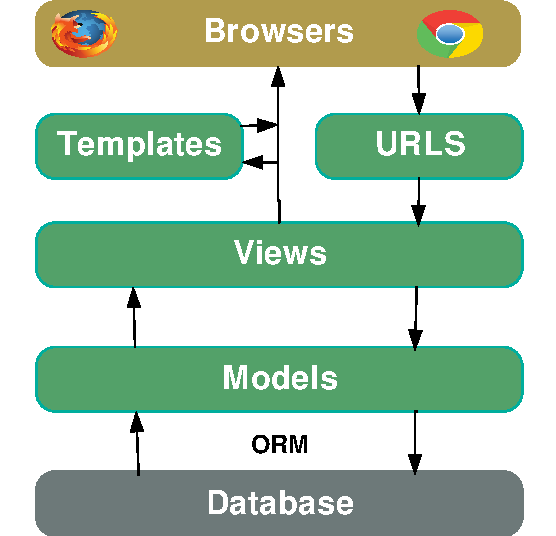
\includegraphics[scale=0.7]{fluxo_django}  %pode alterar o tamanho
			\caption[Fluxo de Informações entre Usuário e Aplicação Django]{\label{fig:fluxo_django}Fluxo de Informações entre Usuário e Aplicação Django. Adaptado de: \url{https://github.com/fga-gpp-mds/00-Disciplina/wiki/Padr\%C3\%B5es-Arquiteturais---MVC-X-Arquitetura-do-Django}}
		\end{center}		
	\end{figure}
	
	A criação de um novo projeto django é feita através do comando startproject. O comando exibido no \autoref{cod:start_project} cria um projeto chamado WebSite. O projeto criado contém alguns arquivos pré-configurados como o arquivo wsgi.py, e o settings.py. O primeiro implementa o Web Server Gateway Interface (WSGI), uma especificação que permite que a aplicação desenvolvida possa ser executada em múltiplos servidores web \cite{klaus2012}; o segundo contém configurações gerais de um site, como por exemplo, qual será o banco de dados utilizado, caminho dos arquivos estáticos, etc.
	
	\begin{listing}[!htb]
		\begin{minted}[bgcolor=bg,breaklines=true,tabsize=2, baselinestretch=1,fontsize=\footnotesize]{bash}
		# navegue até o diretóio destino da aplicação
		$ django-admin startproject WebSite
		\end{minted}
		\caption{Função que interpreta comandos vindos do WebServer}
		\label{cod:start_project}
	\end{listing}
	
	O projeto é constituído de 3 aplicações: core, operation e trend. O funcionamento das mesmas será explicado a seguir:
	
	\subsubsection{Aplicação Core}
	É a aplicação base do sistema. Nesta aplicação são armazenadas todos os arquivos estáticos necessários, como arquivos de imagens, arquivos de estilo (css) e arquivos javascript que são utilizados pelas demais aplicações. Esta aplicação não implementa nenhum modelo de dados, pois sua função é somente servir de sustentação para outras aplicações.
	
	O core possui dois templates: base.html e home.html. O template base consiste na estrutura geral da interface, que possui uma barra de navegação, um espaço central para inserção de conteúdo e um rodapé. Este template é utilizado pelos demais, que apenas preenchem os ``espaços'' disponibilizados no template base, para assim construir uma interface completa. A estrutura do arquivo base é mostrada no \autoref{cod:base}
	
	\begin{listing}[!htb]
		\begin{minted}[bgcolor=bg,breaklines=true,tabsize=2, baselinestretch=1,fontsize=\footnotesize]{django}
		<1 - Inicialização da estrutura padrão de um arquivo html>
		<2 - Inicialização de arquivos de estilo css comuns a todos os templates>
		<3 - Espaço para arquivos de estilo adicionais>
		<4 - Código da Barra de navegação>
		<5 - Espaço Central para inserção de conteúdo por outros templates>
		<6 - Código do rodapé>
		<7 - Inicialização de arquivos javascript comuns a todos os templates>
		<8 - Espaço para inserção de arquivos javascript adicionais>
		\end{minted}
		\caption{Template Base}
		\label{cod:base}
	\end{listing}
	
	O template home.html implementa a página inicial do sistema, que é composta por duas imagens. O template home reutiliza o template base e preenche o espaço de conteúdo disponível. Não adiciona nenhum arquivo javascript ou css. O arquivo urls possui o mapeamento para apenas uma função no arquivo views, que é a chamada para a página inicial.
	
	\subsubsection{Aplicação Operation}
	A aplicação operation contém o maior número de funcionalidades do projeto. Nesta aplicação, são apresentadas para o usuário as informações sobre as variáveis que representam o estado do trocador de calor, bem como estão disponíveis os componentes que permitem a intervenção do usuário sobre o sistema. Ou seja, essa interface contém basicamente displays,para exibir informações, e botões para enviar comandos do usuário para o sistema.
	
	Foram criados 3 modelos de dados para essa aplicação. Como mencionado na \autoref{sec:django}, cada modelo de dados é mapeado em uma tabela no banco de dados. O modelo Display define uma estrutura de dados para exibição de dados analógicos. Através dessa definição, torna-se fácil alterações na unidade de engenharia, texto de descrição, entre outros fatores. O modelo Registers, é definido como o conjunto de informações enviadas pelo Arduino, ou seja, cada linha dessa tabela define o estado do trocador de calor em um dado instante. O modelo OperationMode consiste em armazenar informações auxiliares, como por exemplo se o armazenamento histórico está habilitado ou não. O mapeamento dessas estruturas no banco de dados está resumido na \autoref{tbl7}.
	
	\begin{table}[!htb]
		\centering
		\caption{Modelos definidos no sistema}
		\label{tbl7}
		\def\arraystretch{1.3}
		\resizebox{\textwidth}{!}{
			\begin{tabular}{l |c c | c}
				\hline
				\multicolumn{1}{c|}{\textbf{Displays}} & \multicolumn{2}{c |}{\textbf{Registers}} &
				\multicolumn{1}{c}{\textbf{OperationMode}} \\ \hline
				
				name: string & TimeStamp: DateTime & ColdFlow: float  & OpMode: bool \\
				UE: string  & Temp1: float & PumpStatus: bool & TrendStarted: bool    \\ 
				description: string & Temp2: float & HeaterStatus: bool &  \\
				Tag: string  & Temp3: float & ArduinoMode: bool &      \\
				Value: float & Temp4: float & EmergencyMode: bool &\\
				& HotFlow: float & PumpSpeed: float & \\
				
				\hline
		\end{tabular}}
	\end{table}
	
	Essa aplicação possui 5 funções definidas na view. A função main, que é acionada quando o usuário clica para entrar nessa tela. Enquanto o usuário se mantiver nessa tela, o navegador envia requisições constantes de atualização dos dados. Essa requisição de atualização chama a função refresh, que retorna para o cliente um pacote JSON com os dados mais atuais do sistema. Essa requisição é feita via AJAX\footnote{Funcionamento do AJAX: \url{https://www.w3schools.com/xml/ajax_intro.asp}}, ou seja, não provoca a atualização de toda a página, apenas dos elementos que necessitam ser atualizados, o que otimiza a performance do sistema.
	
	Quando o usuário clica em algum botão (desde que esteja habilitado), é chamada a view command, que repassa o comando para o gateway; quando o usuário movimenta o slider é chamada a view analogcommand, que repassa o comando de alteração de velocidade da bomba para o gateway. Por fim, a view export\_csv, envia os dados históricos armazenados no banco para o usuário, quando solicitado.
	
	A aplicação possui apenas um template, que reutiliza o template base e preenche o espaço de conteúdo. Para que o template funcione corretamente, foi necessário utilizar alguns arquivos css e javascript extras. A lista de arquivos e sua respectiva utilidade é descrita na \autoref{tbl8}. 
	
	Para que cada botão consiga enviar o respectivo comando para a view, criou-se um parâmetro em cada botão que recebe um índice de comando. Os números atribuídos são os mesmos definidos na \autoref{tbl:comandos}. Os comandos definidos nessa tabela se referem apenas a comandos enviados para o Arduino. Existem ainda outros 3 comandos que são enviados para o gateway: habilitar / desabilitar o armazenamento de dados, e apagar os dados históricos do banco. Para esses botões foram atribuídos índices sequenciais a partir do último número presente na \autoref{tbl:comandos}. Em todos os botões, os índices de comando são do tipo char.
	
	\begin{table}[!htb]
		\centering
		\caption{Arquivos extras utilizados pela aplicação}
		\label{tbl8}
		\def\arraystretch{1.3}
		\begin{tabular}{l p{11cm}}
			\hline
			\multicolumn{1}{c}{\textbf{Arquivo}} & \multicolumn{1}{c }{\textbf{Função}} \\ \hline
			bootstrap-slider.css & Biblioteca mantida por \textcite{rohit2017}, \\
			bootstrap-slider.js & que implementa o objeto slider da aplicação \\ \hline
			raphael-2.1.4.js & Biblioteca mantida por
			\textcite{bojan2016}, que implementa \\
			justgage.js & o objeto gauge (barra de nível circular) da aplicação \\ \hline
			bootstrap-confirmation.js & Biblioteca mantida por \textcite{damien2017} que implementa a confirmação após clique de botões \\ \hline
			operation.js & Arquivo que executa a solicitação cíclica de dados para o servidor, bem como interpreta o retorno e atualiza a página para o usuário. Também monitora os eventos dos botões, e quando algum evento ocorre, envia os comandos para o servidor. \\		
			
			\hline
		\end{tabular}
	\end{table}

	\subsubsection{Aplicação Trend}
		A aplicação trend basicamente exibe os dados analógicos em forma gráfica. Foram definidos 4 gráficos, para separar a visualização das grandezas. A relação entre as grandezas e em qual gráfico está exibida é mostrada \autoref{tbl:area_chart}.
		
		\begin{table}[!htb]
			\centering
			\caption{Arquivos extras utilizados pela aplicação}
			\label{tbl:area_chart}
			\def\arraystretch{1.3}
			\begin{tabular}{c p{7 cm}}
				\hline
				\textbf{Índice Área} & \multicolumn{1}{c}{\textbf{Grandezas}} \\ \hline
				1 & Temperaturas do Ciclo de Água Quente \\
				2 & Temperaturas do Ciclo de Água Fria \\
				3 & Vazões de Água Quente e Fria \\
				4 & Velocidade da Bomba \\
				\hline
			\end{tabular}
		\end{table}
	
	Foi criado apenas 1 modelo para essa aplicação. O modelo TrendRegister é praticamente igual ao Register, porém não possui os campos digitais, apenas os analógicos. 
	
	A aplicação possui apenas 2 funcões definidas no arquivo view. A função main, é acionada quando o usuário clica para entrar na tela. Enquanto o usuário se mantiver nessa tela, o navegador envia requisições constantes de atualização de dados. Ou seja, nesse quesito funciona de forma idêntica à aplicação operation descrita anteriormente.
	
	Para implementar a visualização em forma gráfica, foi necessário implementar bibliotecas de terceiros. Existem algumas bibliotecas open-source para exibir dados de forma gráfica na internet. A biblioteca escolhida foi a ``SmoothieCharts'', disponibilizada por \textcite{walnes2017}.
	
	O template dessa aplicação utiliza o template base e preenche o espaço central com os gráficos. Basicamente, o arquivo contém a definição das 4 áreas que serão exibidos os gráficos e adiciona dois arquivos javascript. O primeiro deles é a biblioteca mencionada anteriormente, e o segundo é o arquivo trend.js, que controla a frequência de requisição de dados para o servidor, bem como utiliza as funções disponibilizadas pela biblioteca para implementar a animação do gráfico.
		